\chapter{Evaluation}

\section{Aims}

In this chapter, we look to assess aims we presented at the beginning of this work where we claimed to use reinforcement learning to perform automated optimisation of deep learning computation graphs. Thus, this evaluation seeks to answer the following questions:

\begin{enumerate}
  \item Are model-based reinforcement learning methods able to model the transition dynamics of the environment?
  \item Is the agent policies able to generalise to unseen states of the same graph to act in accordance to our performance objectives?
  \item Do the world models accurately model the reward estimation from the graphs latent state?
  \item Are the agents trained in an imagined world model applicable to the real-world environment?
\end{enumerate}

Throughout this chapter, we aim to answer these questions by a series of experiments which provide evidence to support our claims. Finally, we conclude with an overall discussion of our findings and its impact.

\section{Experimental Setup}

All the experiments presented in this chapter, both training various agent models and testing, is performed using the codebase available in the GitLab repository for this project \footnote{\url{https://www.gitlab.com/CamRL/xflowrl}}. The project was developed, and the experiments were performed using a single machine running Ubuntu Linux 18.04 with a 6-core Intel i7-10750H@2.6GHz, 16GB RAM and an NVIDIA GeForce RTX 2070.

To interface with the internal representation of the computation graphs, as previously discussed, we used the open-sourced version of TASO \cite{jia2019taso} which we modified to extract detailed runtime information. Further, we implemented the reinforcement learning algorithms in TensorFlow 2 \cite{tensorflow2015-whitepaper} and utilised the \texttt{graph\textunderscore nets} package developed by Battaglia et al. \cite{battaglia2018relational} to process our input graphs which we described in chapter \ref{sec:prob:subsec:sysenv}. The PPO agent was implemented based upon the implementation provided by Schulman et al. \cite{schulman2017proximal}.

\subsection{Graphs Used}
\label{sec:eval:subsec:graphsused}

\begin{table}[htbp]
  \centering
  \resizebox{\columnwidth}{!}{
    \begin{tabular}{@{}llllll@{}}
      \toprule
                    & InceptionV3   & ResNet-18     & ResNet-50     & SqueezeNet1.1 & BERT        \\ \midrule
      Type          & Convolutional & Convolutional & Convolutional & Convolutional & Transformer \\
      Layers        & 43            & 18            & 50            & 21            & 12          \\
      Unique Layers & 12            & 6             & 6             & 3             & 3           \\
      Substitutions & 56            & 40            & 228           & 288           & 80          \\ \bottomrule
      \end{tabular}
  }
  \caption[Properties of evaluation graphs]{Properties of the five evaluation graphs used in the experiments contained in this chapter. We differentiate the total number of layers in a network from the number of unique layers used in composing the network to provide a more accurate representation of its complexity.}
  \label{table:eval:graph-props}
\end{table}

We chose to use five real-world deep learning models to evaluate our project. InceptionV3 \cite{szegedy2015rethinking} is a common, high-accuracy model for image classification trained on the ImageNet dataset \footnote{\url{https://image-net.org/index.php}}. ResNet-18 \& ResNet-50 \cite{he2015deep} are also deep convolutional networks that are 18 and 50 layers deep respectively. SqueezeNet \cite{iandola2016squeezenet} is a shallower yet accurate model on the same ImageNet dataset. BERT \cite{devlin2019bert} is a recent large transformer network that has been to improve Google search results \cite{nayak2019}. As these graph were also used in the evaluation of TASO \cite{jia2019taso}, we can show a direct comparison of the performance between the different approaches.

\section{Experiments}

%\subsection{Hyperparameter Selection}
%[TODO]

\subsection{Baselines}
\label{sec:eval:subsec:baseline}

In this section, we will establish the baseline performance results from prior work and modern machine learning frameworks such that we can compare against our proposed approach and quantitatively analyse the results. We show the runtime metrics of the five graphs described in section \ref{sec:eval:subsec:graphsused} that are optimised using TensorFlow \cite{tensorflow2015-whitepaper}, TensorRT \cite{tensorrt2017} and TASO \cite{jia2019taso}.

% Baselines (TASO, TensorFlow, TVM etc)

\begin{figure}[h]
  \centering
  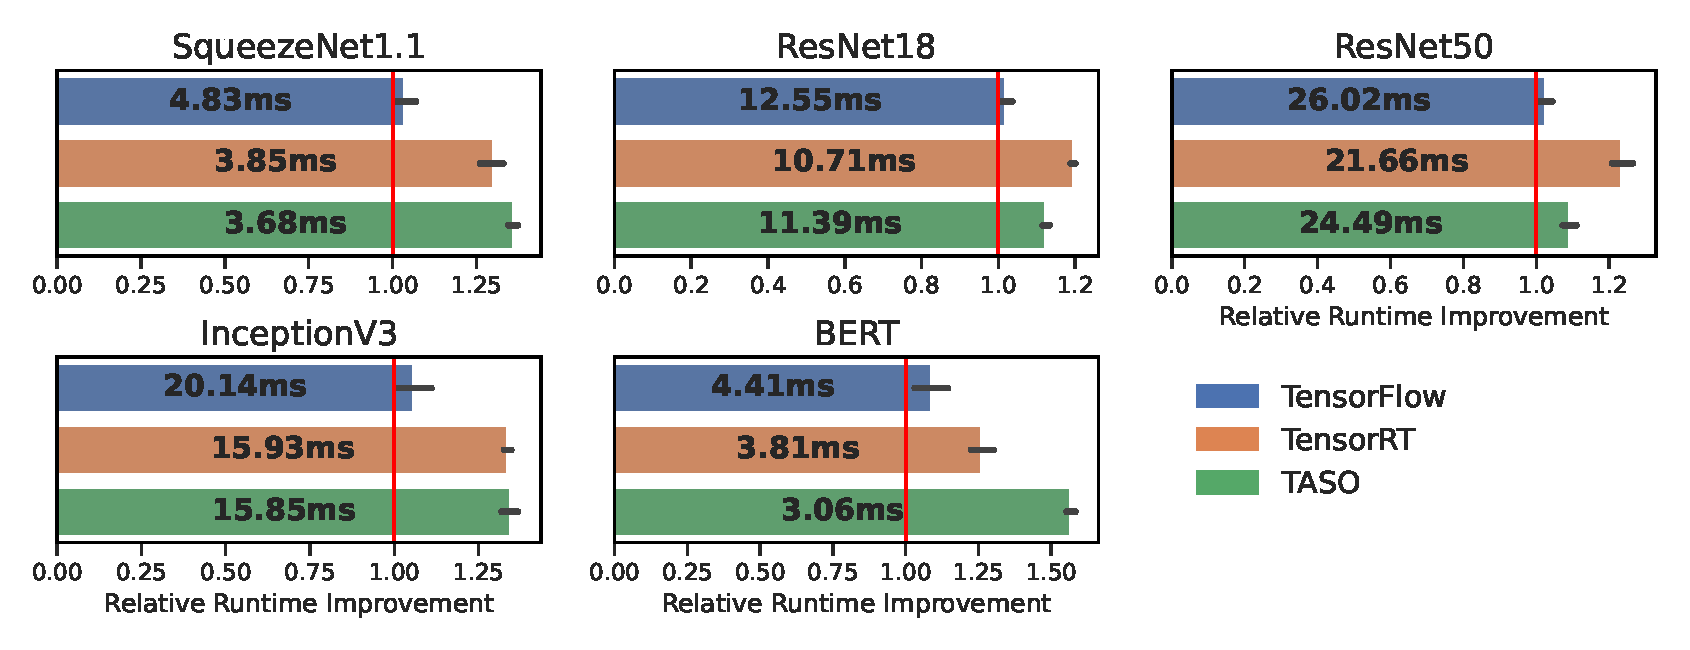
\includegraphics[width=1\columnwidth]{sections/5evaluation/images/runtimes_baseline_h}
  \caption[Baseline runtimes of optimised graphs]{Runtime of optimised graphs using the three baseline optimisation methods. The x-axis shows the relative runtime improvement, a higher relative runtime is better.}
  \label{fig:eval:baseline-runtimes}
\end{figure}

Figure \ref{fig:eval:baseline-runtimes} shows the runtime of each optimised graph described in section \ref{sec:eval:subsec:graphsused} using the three baseline methods, TensorFlow \cite{tensorflow2015-whitepaper}, TensorRT \cite{tensorrt2017} and TASO \cite{jia2019taso}. We observe that TASO outperforms TensorFlow Grappler and TensorRT on BERT by 50.5\% and 43.6\% respectively. On the other hand, with convolutional networks, the optimised graph discovered by TASO has a runtime within $\pm 6$\% compared to TensorRT. Furthermore, we note that during our reproduction of the results found by Jia et al. \cite{jia2019taso}, we used the same value of $\alpha = 1.05$ and a search budget of 50,000 steps. TASO often found the optimal graph within $\sim$5000 steps and the remaining computation steps failed to further improve the estimated runtime.

\begin{figure}[h]
  \centering
  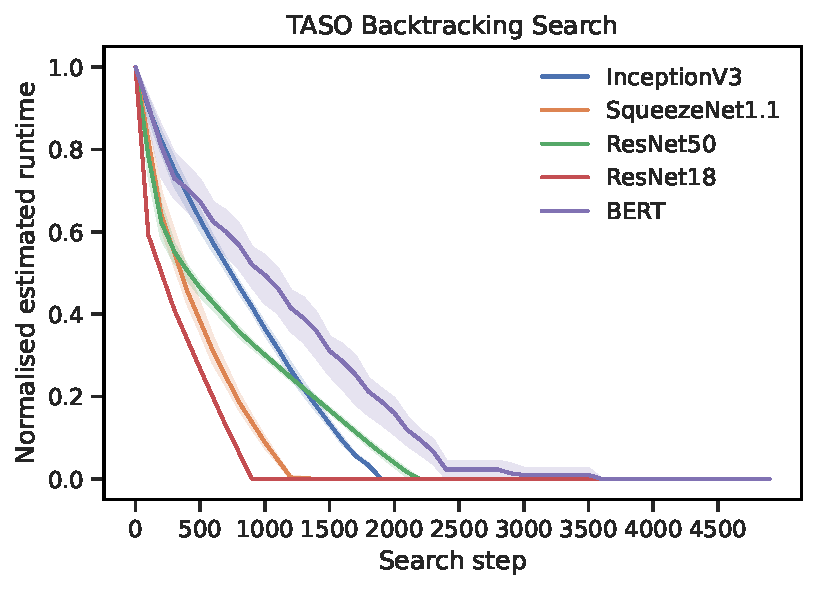
\includegraphics[width=1\columnwidth]{sections/5evaluation/images/taso_graph_search}
  \caption[TASO backtracking search]{We show the estimated runtime improvement, normalised between the minimum and maximum obtained runtimes, for each tested graph. We performed each experiment five times and show the 95\% confidence interval for each graph. We also note that we clipped the plot as after 5000 steps, there was no increase in performance for the remaining 45000 search steps.}
  \label{fig:eval:baseline-taso-search}
\end{figure}

Figure \ref{fig:eval:baseline-taso-search} shows a plot of the runtime estimated by TASO at each step in the search. We repeated each experiment five times and show the confidence interval for each graph. Based upon the results, we observe that TASO did not just take the longest to discover the optimised graph, the variance between runs was the highest compared to other graphs. One reason for this disparity is that it has a vastly different architecture; BERT is a transformer network which, compared to convolution networks, has a greater breadth than depth. As such, when TASO performs the backtracking search, there are far more initial locations in the graph where a substitution can be applied.

\subsection{Model-Free Agent}
\label{sec:eval:subsec:mfagent}

In this section we describe our experiments performed using the model-free agent which acts inside the real environment. Firstly, we trained the agent on each graph under consideration and evaluated its optimised runtime, the results of which we present in figure \ref{fig:eval:mf-agent-runtimes}. In the worst case, the model-free agent performs a series of optimisations that increases runtime by 9\% compared to those discovered by TASO.

\begin{figure}[h]
  \centering
  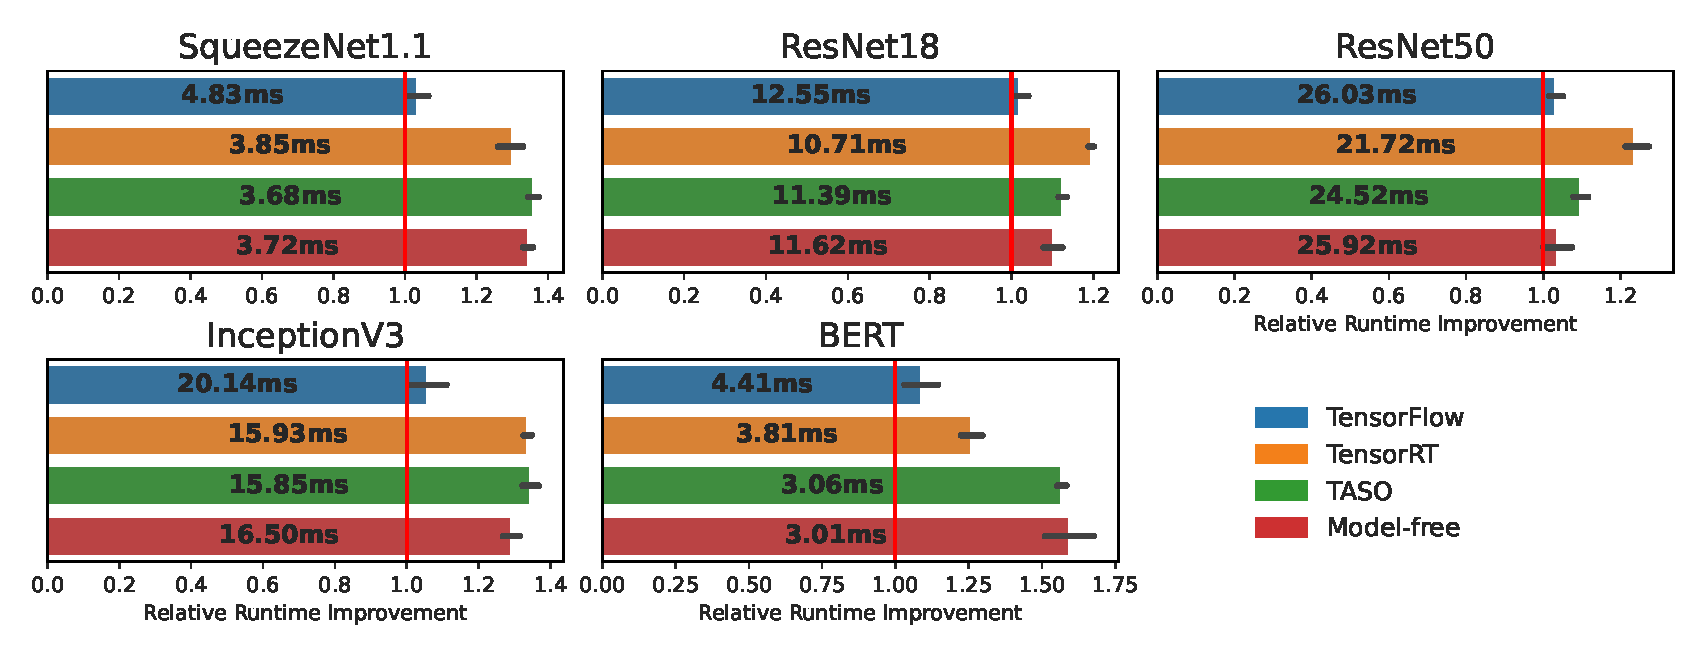
\includegraphics[width=1\columnwidth]{sections/5evaluation/images/runtimes_mf_h}
  \caption[Runtimes of optimised graphs using MF-RL]{Runtime of optimised graphs using an agent trained using the model-free PPO algorithm. We also show the baseline results as comparison. The x-axis shows the relative runtime improvement, a higher relative runtime is better.}
  \label{fig:eval:mf-agent-runtimes}
\end{figure}

\begin{figure}[h]
  \centering
  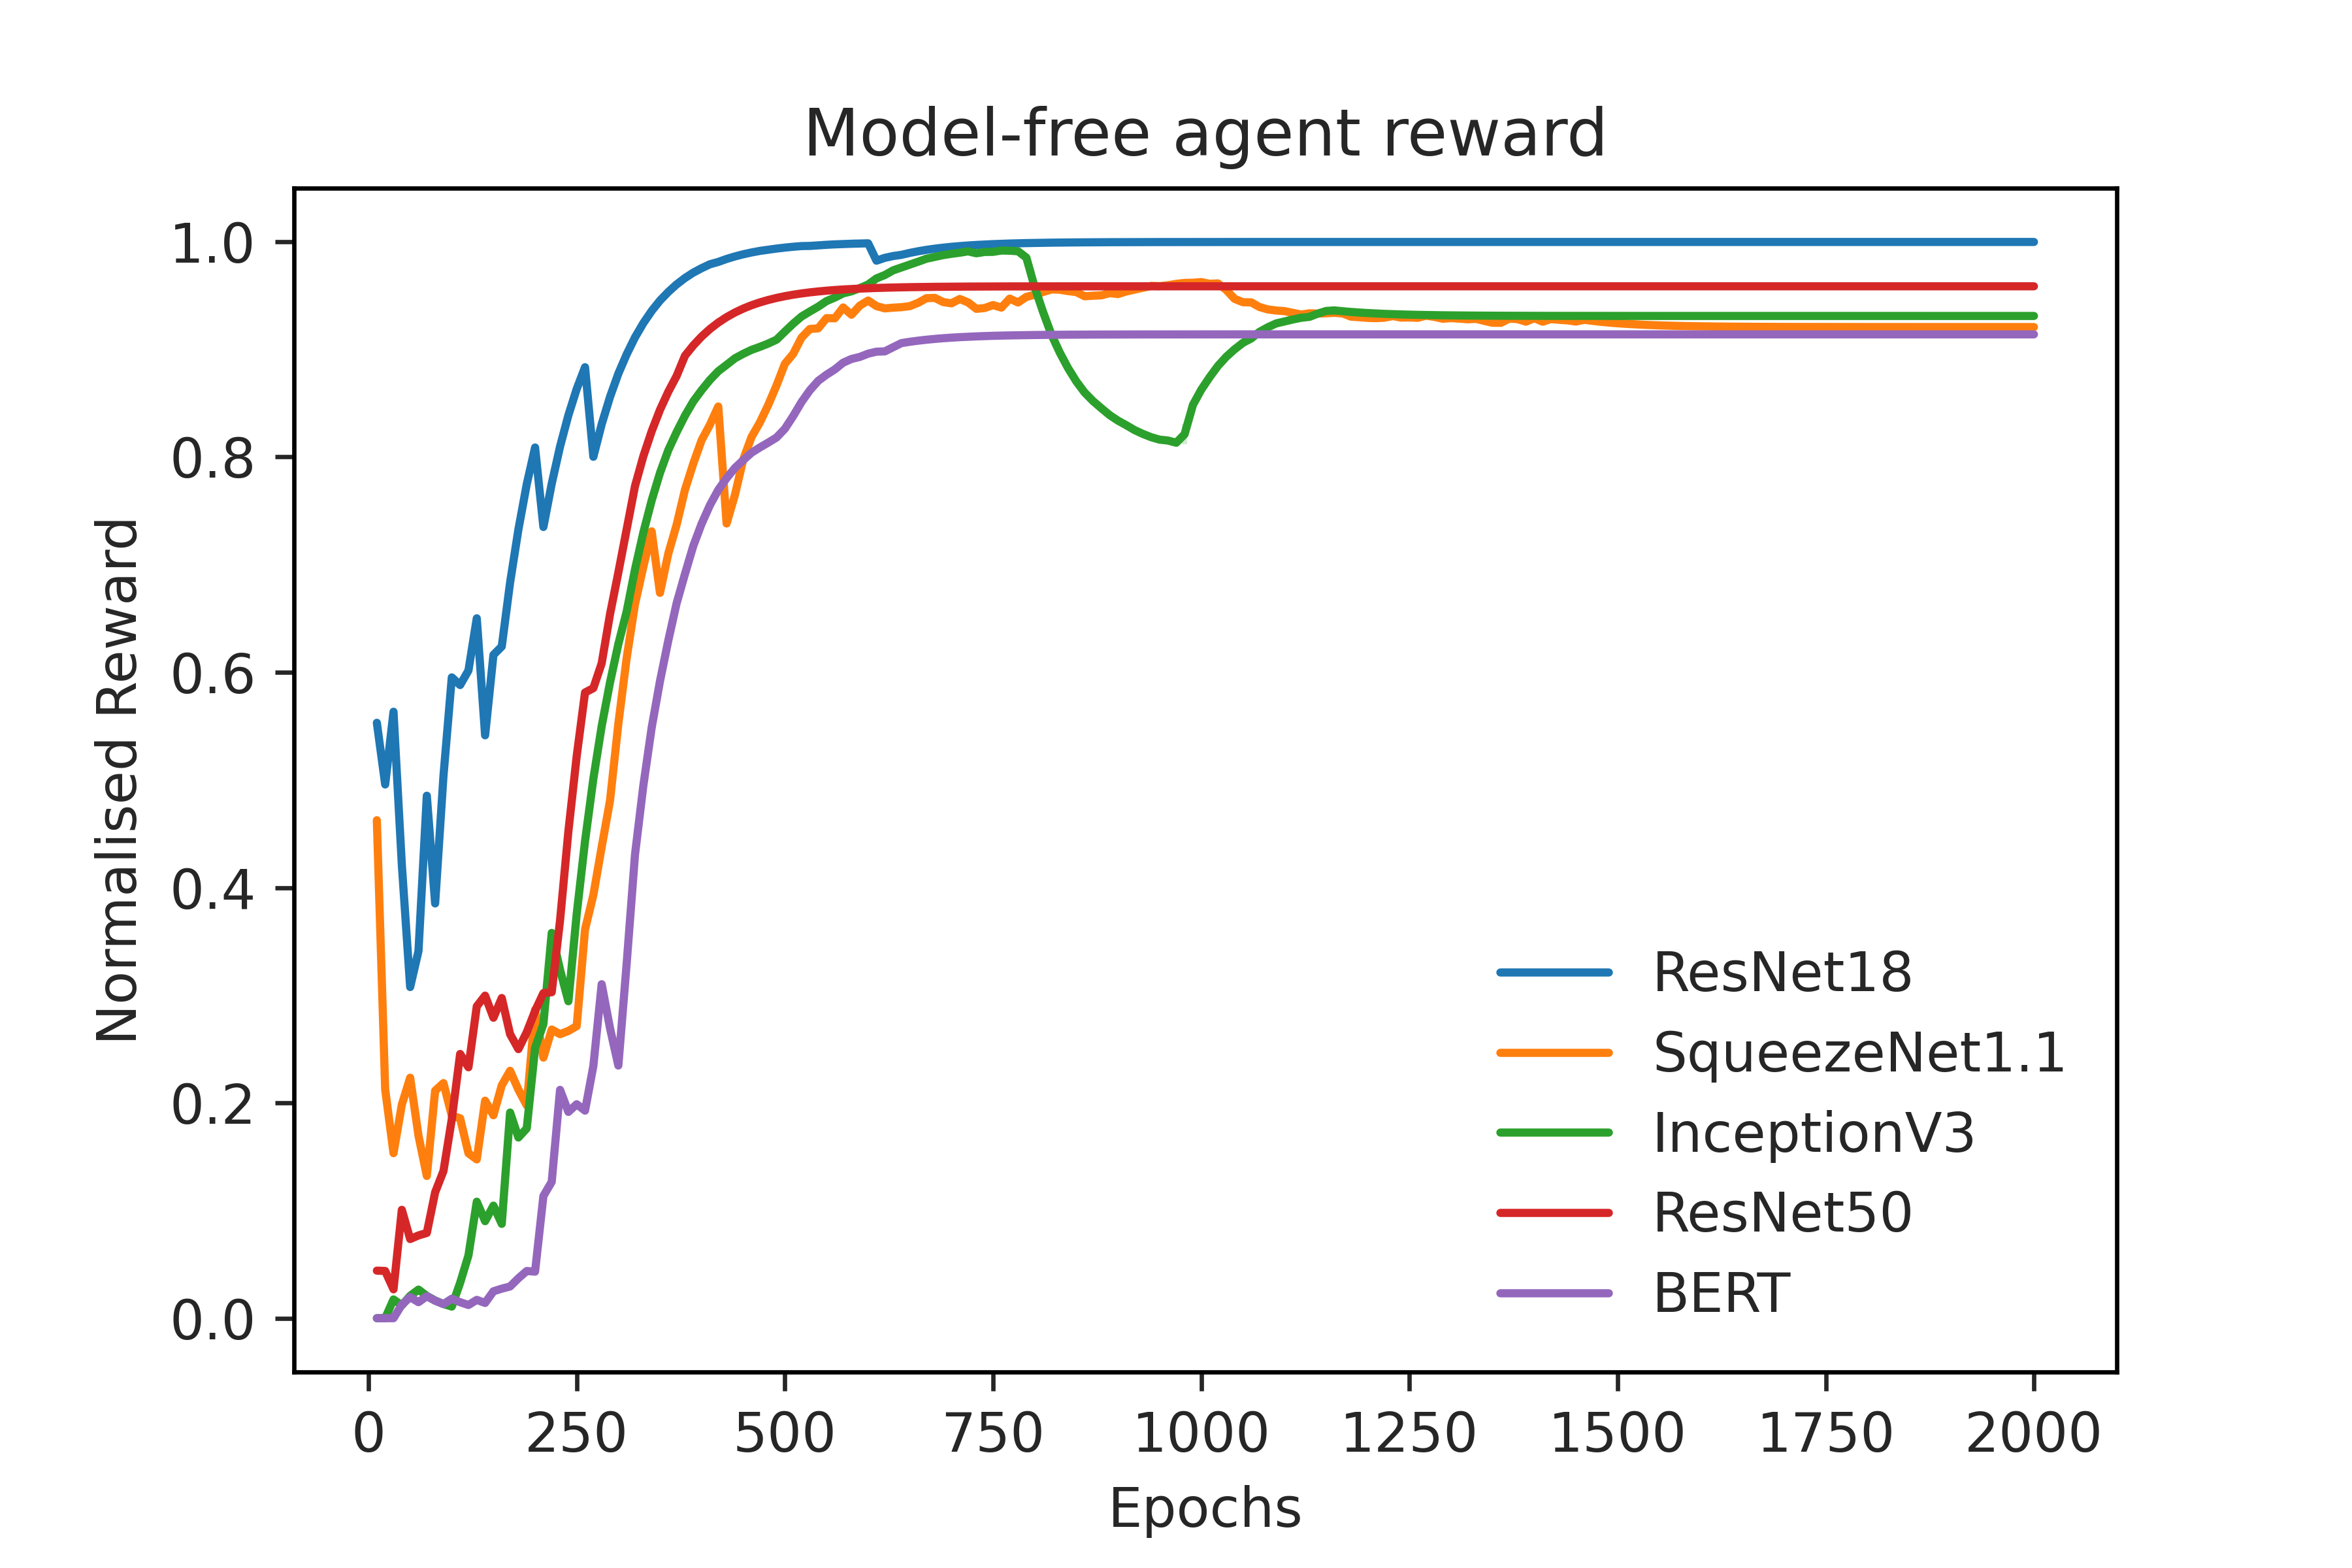
\includegraphics[width=1\columnwidth]{sections/5evaluation/images/mf_training_reward}
  \caption[Epoch reward during training of model-free agent]{Normalised reward of model-free agent produced by the real environment in response to selected actions by the agent}
  \label{fig:eval:mf-agent-reward}
\end{figure}

Figure \ref{fig:eval:mf-agent-reward} shows the reward produced by the model-free agent acting inside the real environment for each graph. Due to the difference in estimated runtime between graphs, we used min-max normalisation to scale the rewards into the same range. First and foremost, it is evident that the graph optimisation using the model-free agent reward converge quickly after only $\sim$1000 epochs with low variation in the average epoch rewards after convergence.

\subsubsection{Reward functions}
\label{sec:eval:subsec:mf:subsubsec:rwd-func}

As we described in section \ref{sec:prob:subsec:rwd}, the design of the reward function used in the training of RL agents is a pivotal part of the agents architecture. In this section, we analyse our proposed reward functions and the effect on the convergence as well as final performance of the trained agents.

\begin{figure}[htbp]
  \centering
  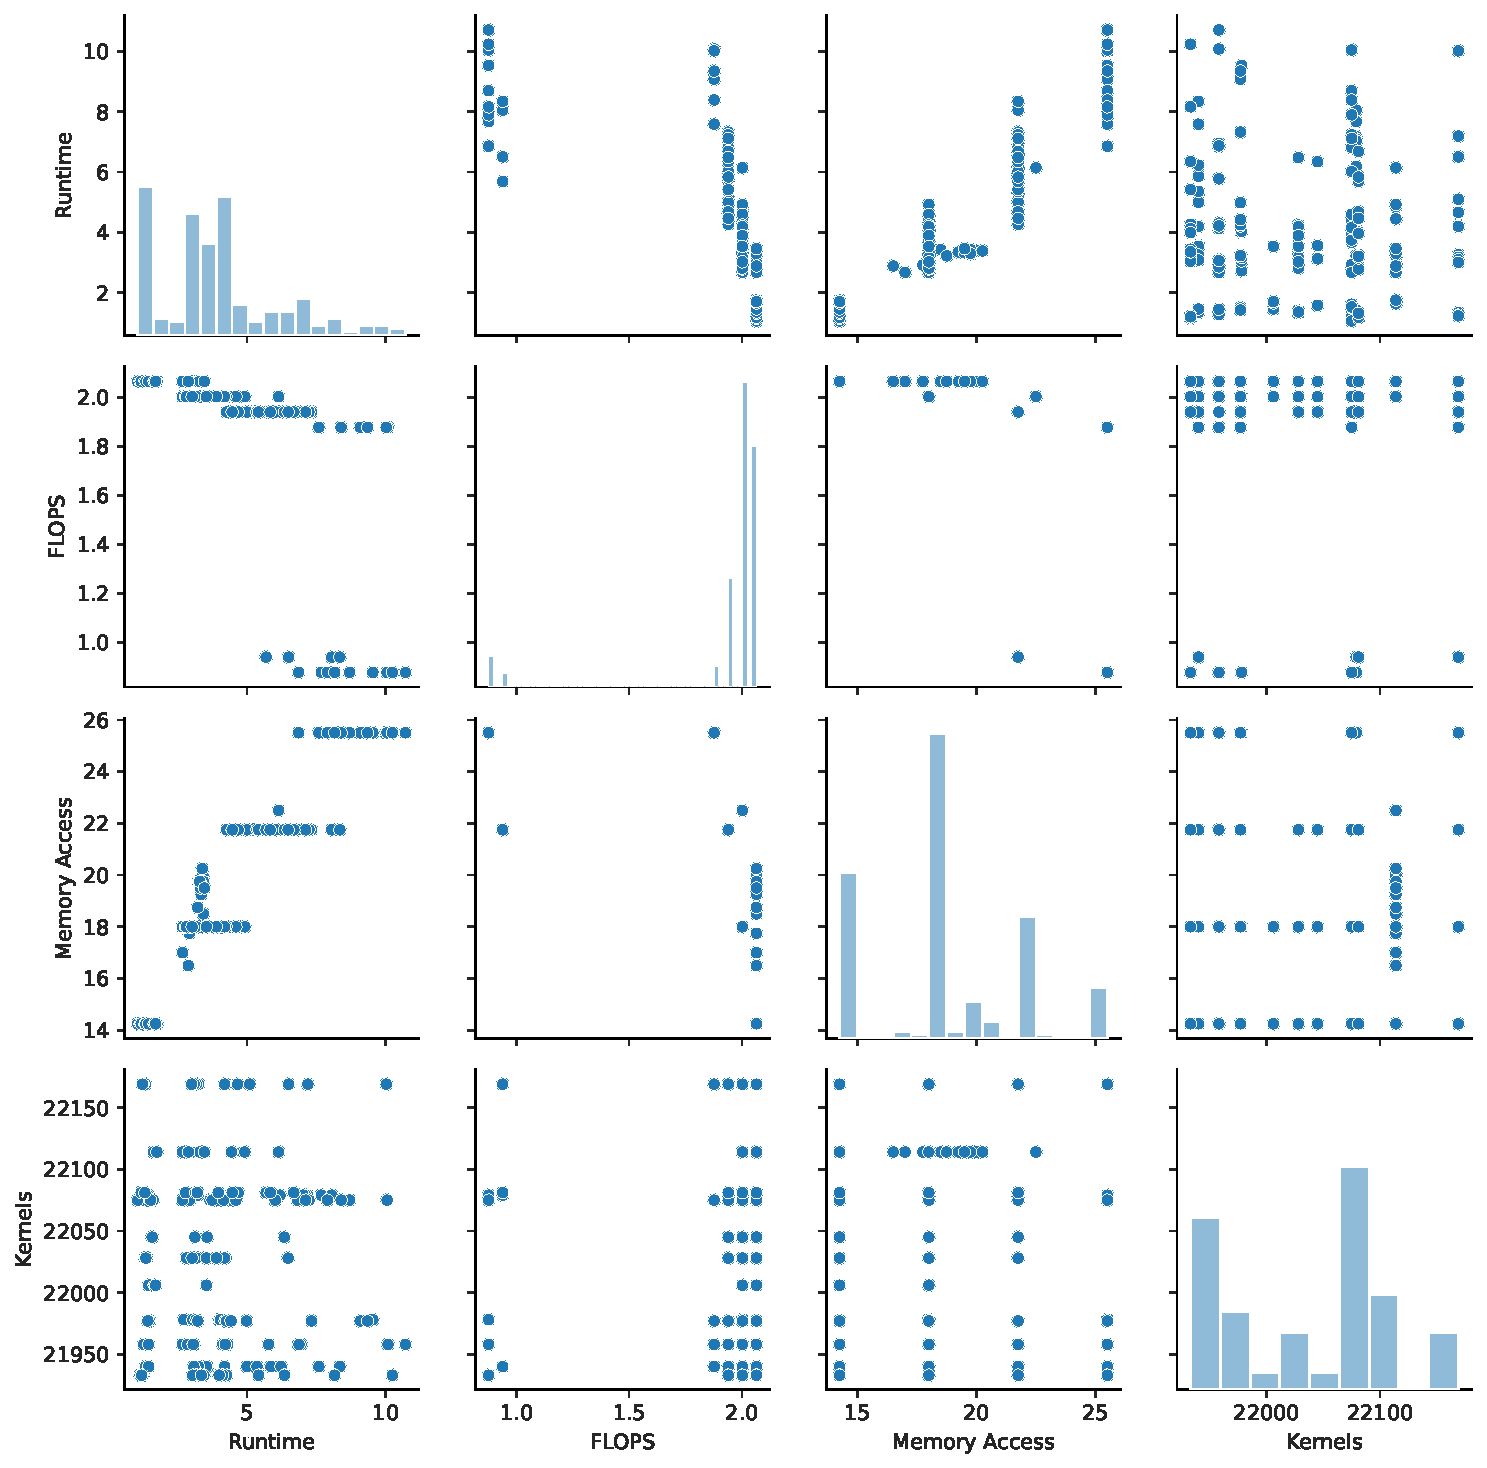
\includegraphics[width=1\columnwidth]{sections/5evaluation/images/pairplot_bert.pdf}
  \caption[Pairwise plot of correlation between runtime metrics]{We show the pairwise correlation between the detailed runtime metrics recorded directly from the TASO environment while training on the BERT graph. We note the strong correlation between the number of memory accesses and estimated runtime improvement.}
  \label{fig:eval:pairplot-bert}
\end{figure}

Figure \ref{fig:eval:pairplot-bert} shows the pairwise relationship between the four detailed runtime measurements which we record at each step of the training process for the BERT graph. We collected the runtime, FLOPS, memory access and number of kernel launches and show the relationship between the values. We note that the estimated runtime and memory accesses have a strong correlation; when the memory access decreases, we see a notable decrease in estimated runtime. 

\begin{figure}[h]
  \centering
  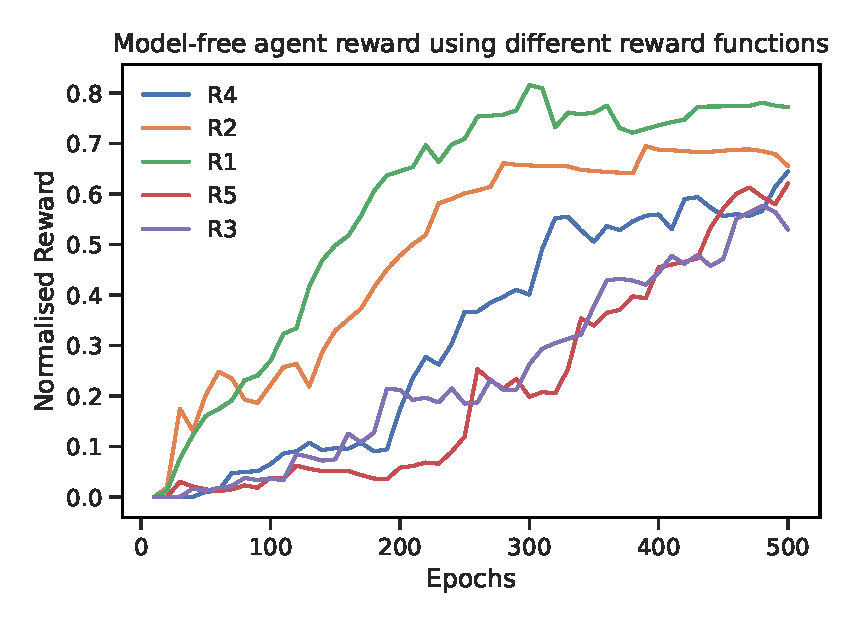
\includegraphics[width=1\columnwidth]{sections/5evaluation/images/mf_reward_func.eps}
  \caption[Agent reward using various reward functions]{We show the normalised reward of each agent using various reward functions while being trained for 500 epochs. R1 uses the second reward function with tuned parameters, R2 uses new runtime reward, R3 uses $\alpha=0.1, \beta=0.9$, R4 uses $\alpha=0.5, \beta=0.5$ and finally, R5 uses incremental runtime improvement.}
  \label{fig:eval:mf-reward-funcs}
\end{figure}

Figure \ref{fig:eval:mf-reward-funcs} shows the effect on convergence of model-free RL agents while training on the BERT graph using various reward functions. Significantly, using a standard, yet naive approach of the first reward function described in section \ref{sec:prob:subsec:rwd} shows that the model-free agent improves at a linear rate as shown by R4 in figure \ref{fig:eval:mf-reward-funcs}. Whereas, using the second reward function and tuned hyperparameters of $\alpha$ and $\beta$, shown by R1, converges the fastest.

However, the rate of convergence does not show the whole picture of the agents performance. We note that the highest performing agent, after the restricted 500 epoch training time, was R1 with an average runtime improvement of $48.7 \pm 3.2\%$. Surprisingly, the second highest performing agent was the agent using R4, the simplest reward function from the set tested, with a performance of $43.2 \pm 2.3\%$.

In order to find the values of hyperparameters $\alpha$ and $\beta$ which results in the agent with the maximum performance, we performed a grid search for $\alpha$ and $\beta = 1 - \alpha$ between the values of $[0, 1]$; we searched between the bounds in increments of $0.1$. After training each agent for 500 epochs and evaluate the performance of each agent three times, we found that the reward function resulting in the highest performance was using the values $0.8$ and $0.2$ for $\alpha$ and $\beta$ respectively.

\subsection{Model-based Agent}
\label{sec:eval:subsec:mbagent}

In this section we first present the results for training an agent inside a world model for each graph individually. Secondly, we compare the model-based agent performance to baseline measurements as well as showing the change in memory usage which is a by product from the applying graph transformations in order to reduce runtime. Furthermore, we also discuss the impact of hyperparameter selection on the agent performance as well as showing the accuracy of the world model in regards to graph reward prediction.

\subsubsection{Runtime Performance}
\label{sec:eval:subsec:mb:sec:runtimeperf}

Figure \ref{fig:eval:world-model-runtimes} shows the runtime of the optimised graphs for the model-based agents trained inside the fully hallucinogenic world model. Each agent was trained inside a world model using rollouts from its respective graph as described in section \ref{sec:rlopt:subsec:actionctrl}. We trained the agents for a maximum of 1000 epochs, in mini-batches of 10 epochs. Additionally, we used a fixed learning rate for both the policy and value networks during training of the controller agent network.

\begin{figure}[h]
  \centering
  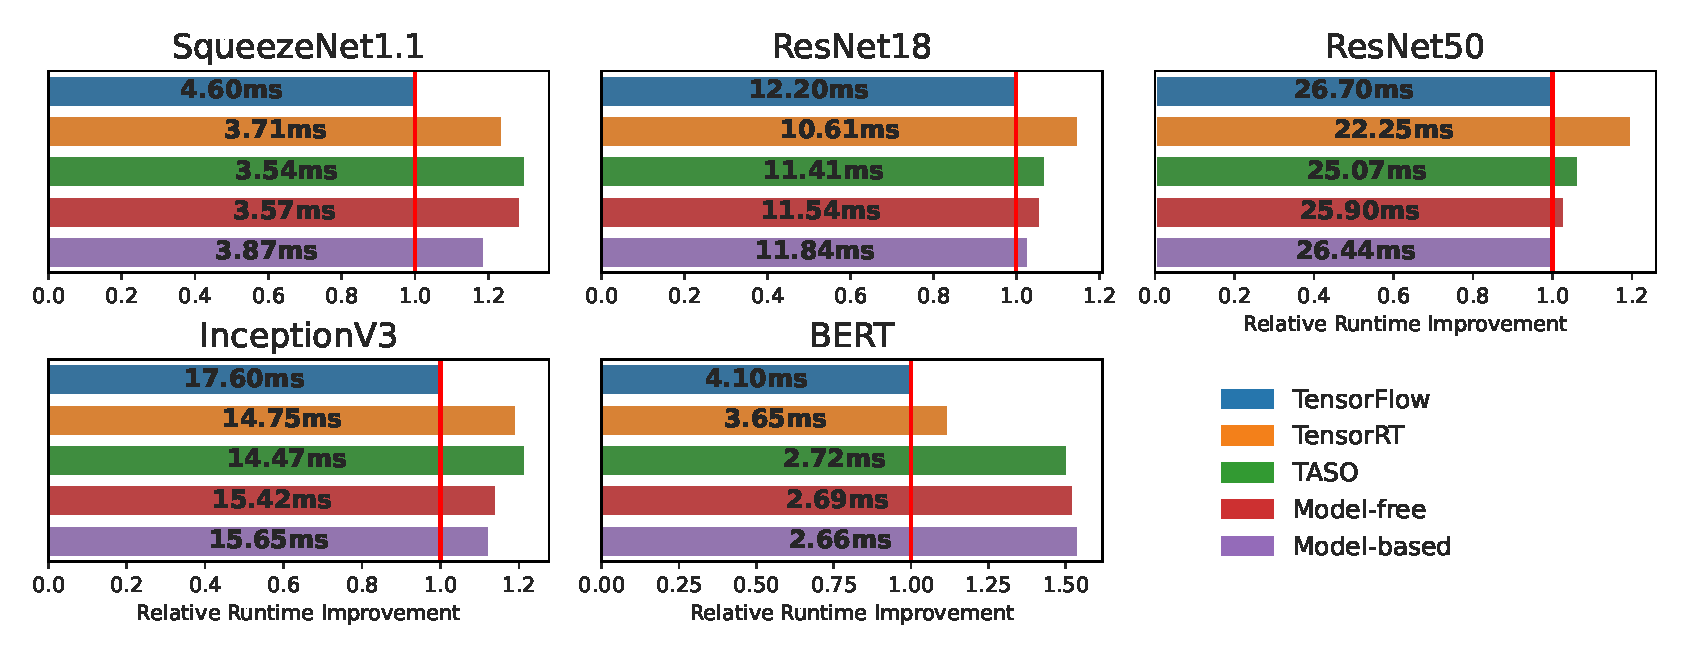
\includegraphics[width=1\columnwidth]{sections/5evaluation/images/runtimes_all_h}
  \caption[Runtimes of optimised graphs using a model-based controller]{Runtime of optimised graphs using an agent trained using the model-based world model. We also show the baseline results as comparison. The x-axis shows the relative runtime improvement, a higher relative runtime is better.}
  \label{fig:eval:world-model-runtimes}
\end{figure}

Firstly, we note that training the agents on convolutional networks, especially SqueezeNet1.1 and InceptionV3, the model-based agent failed to outperform TASO, we still decreased the runtime compared to the baseline graph produced by TensorFlow Grapper. Importantly, we observe that the model-based agent outperformed all baseline approaches on the BERT transformer network; we improved the runtime by 54.1\% and 7.3\% compared to TensorFlow and TASO respectively. Figure \ref{fig:eval:xfer-heatmap} shows the transformations applied by the model-based agent on the test graphs and compared to TASO, we only apply a single transformation over 20 times---compared to TASO which uses four distinct transformations produce the optimised graph.

% [TODO - describe the type of transformations applied to better compare]

Compared to the strictly model-free agent that was trained in the real environment, our model-based agent achieved a similar level of performance in the majority of the tested graphs. The model-free agent was trained for 2000 epochs and, by extension, over 4,000,000 interactions with the real environment. Comparatively, the model-based agent performed approximately 1,000,000 interactions with the real environment as the agent did not interact with the real environment while training inside the world model. Therefore, it is evident that by training inside the world model we improved the sample efficiency of the agent. On the other hand, the performance of the agent decreased compared to the model-free agent in four of the five tested graphs.

Furthermore, an important consideration when training inside a systems environment is the wall-clock time for stepping the environment to a new state based upon the agent action. We analysed the time required to perform a single step while training the ResNet50 graph. We found that stepping the world model (performing inference of the world-model) takes, on average, 10ms whereas stepping the real environment takes on average 850ms. Thus, although the performance of the model-based agent was comparatively lower, our wall-clock time for required for training was reduced by a factor of 85x.

\subsubsection{Optimisation Time}

\begin{figure}[h]
  \centering
  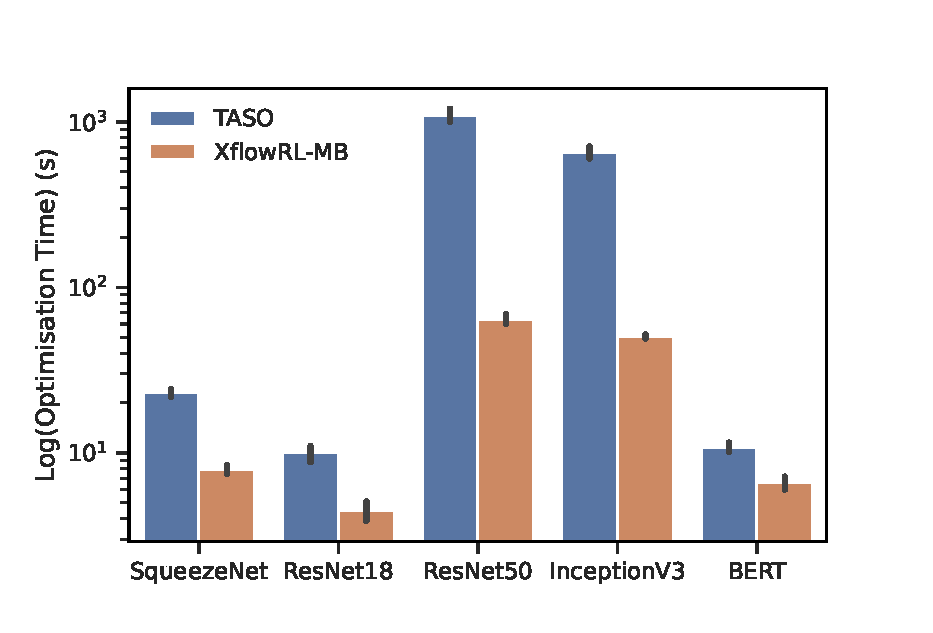
\includegraphics[width=0.75\columnwidth]{sections/5evaluation/images/optimisation_time}
  \caption[Optimisation time for TASO and MB-RL]{Time required to generate the optimised model using  model-based RL and TASO}
  \label{fig:eval:optimisation-time}
\end{figure}

Figure \ref{fig:eval:optimisation-time} shows the optimisation time required to generate the optimised graph of the tested models. We note that the optimisation time for the model-based agent does not include the time required to learn the world model nor training the controller in the environment. The optimisation time is measured as the the wall-clock time to perform $n$ agent steps to generate the optimised graph using our RL agents. Thus, although TASO has a longer optimisation time compared to the RL agent, TASO only requires us to perform the cost-based search a single time.

\subsubsection{Memory Usage}

% Table of memory usage
\begin{table}[htbp]
  \centering
  \resizebox{\columnwidth}{!}{
    \begin{tabular}{@{}ccccc@{}}
      \toprule
      \multicolumn{1}{l}{} & \multicolumn{2}{c}{Baseline (TF)}                                         & \multicolumn{2}{c}{Optimised (MB-RL)} \\ \midrule
      \multicolumn{1}{l}{} & \multicolumn{1}{l}{Inf. time (ms)} & \multicolumn{1}{l}{Mem. usage (GiB)} & \multicolumn{2}{c}{\% Improvement}    \\
      ResNet18      & 12.2 & 1.18 & 3.0\%  & 1.1\% \\
      ResNet50      & 26.7 & 2.34 & 1.0\%  & 0.6\% \\
      InceptionV3   & 17.6 & 2.11 & 12.5\% & 2.3\% \\
      SqueezeNet1.1 & 4.6  & 1.14 & 18.9\% & 1.8\% \\
      BERT          & 4.1  & 0.26 & 54.1\% & 4.5\% \\ \bottomrule
      \end{tabular}
  }
  \caption[Memory usage of optimised graphs]{Relative performance improvement of the graphs optimised by the model-based agent. We show the inference time, and memory used for performing inference on the model.}
  \label{table:eval:graph-mem-usage}
\end{table}

Table \ref{table:eval:graph-mem-usage} shows the percentage improvement of both the inference time and the memory used for performing inference on the optimised models. Importantly, although we tasked the agent to optimise for reducing the runtime of the graphs, we observe an unintended secondary effect of a reduction in memory usage of up to 4.5\% over the baseline TensorFlow model.

\subsubsection{World-model accuracy}
\label{sec:eval:subsubsec:wm-acc}

\begin{figure}[h]
  \centering
  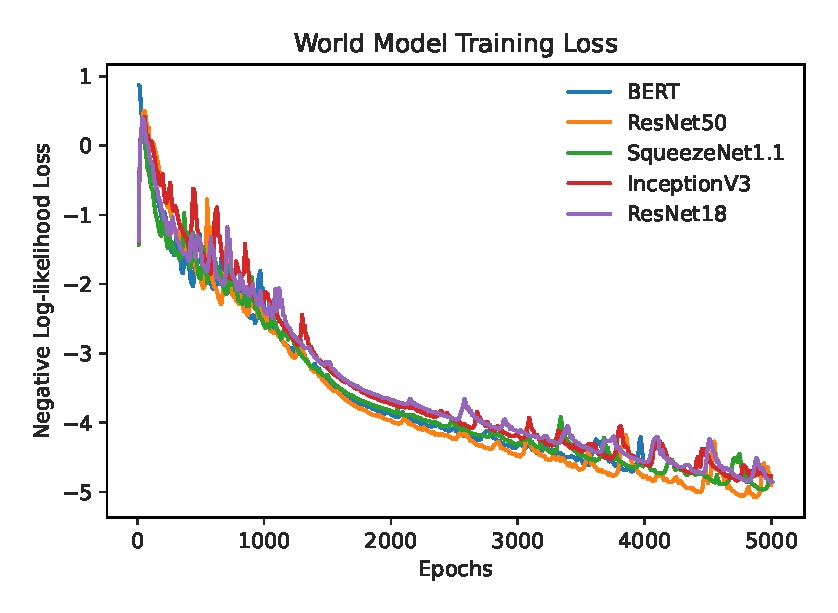
\includegraphics[width=1\columnwidth]{sections/5evaluation/images/mb_training_loss}
  \caption[Log-likelihood loss of world models]{Training plot of the log-likelihood loss for our world model on the five test graphs.}
  \label{fig:eval:world-model-loss}
\end{figure}

The training of the model-based agent is split into two parts. First, we train the world-model, the network that learn to simulate the environment dynamics, and secondly, we train the controller network inside the world-model. In this section, we show the convergence of the world model during training in figure \ref{fig:eval:world-model-loss}. The figure is a plot of the log-likelihood loss per training epoch for each graph. We used the same hyperparameters for training each world model as well as decaying the learning rate over the course of 2000 epochs with a 2nd-degree polynomial decay policy. The MDN-RNN is trained with 8 Gaussians and 256 hidden units, all other hyperparameters used in training the MDN-RNN world model are the same as those used by Ha and Schmidhuber \cite{ha2018worldmodels}, unless otherwise stated.

% TODO explain more!

\begin{figure}[h]
  \centering
  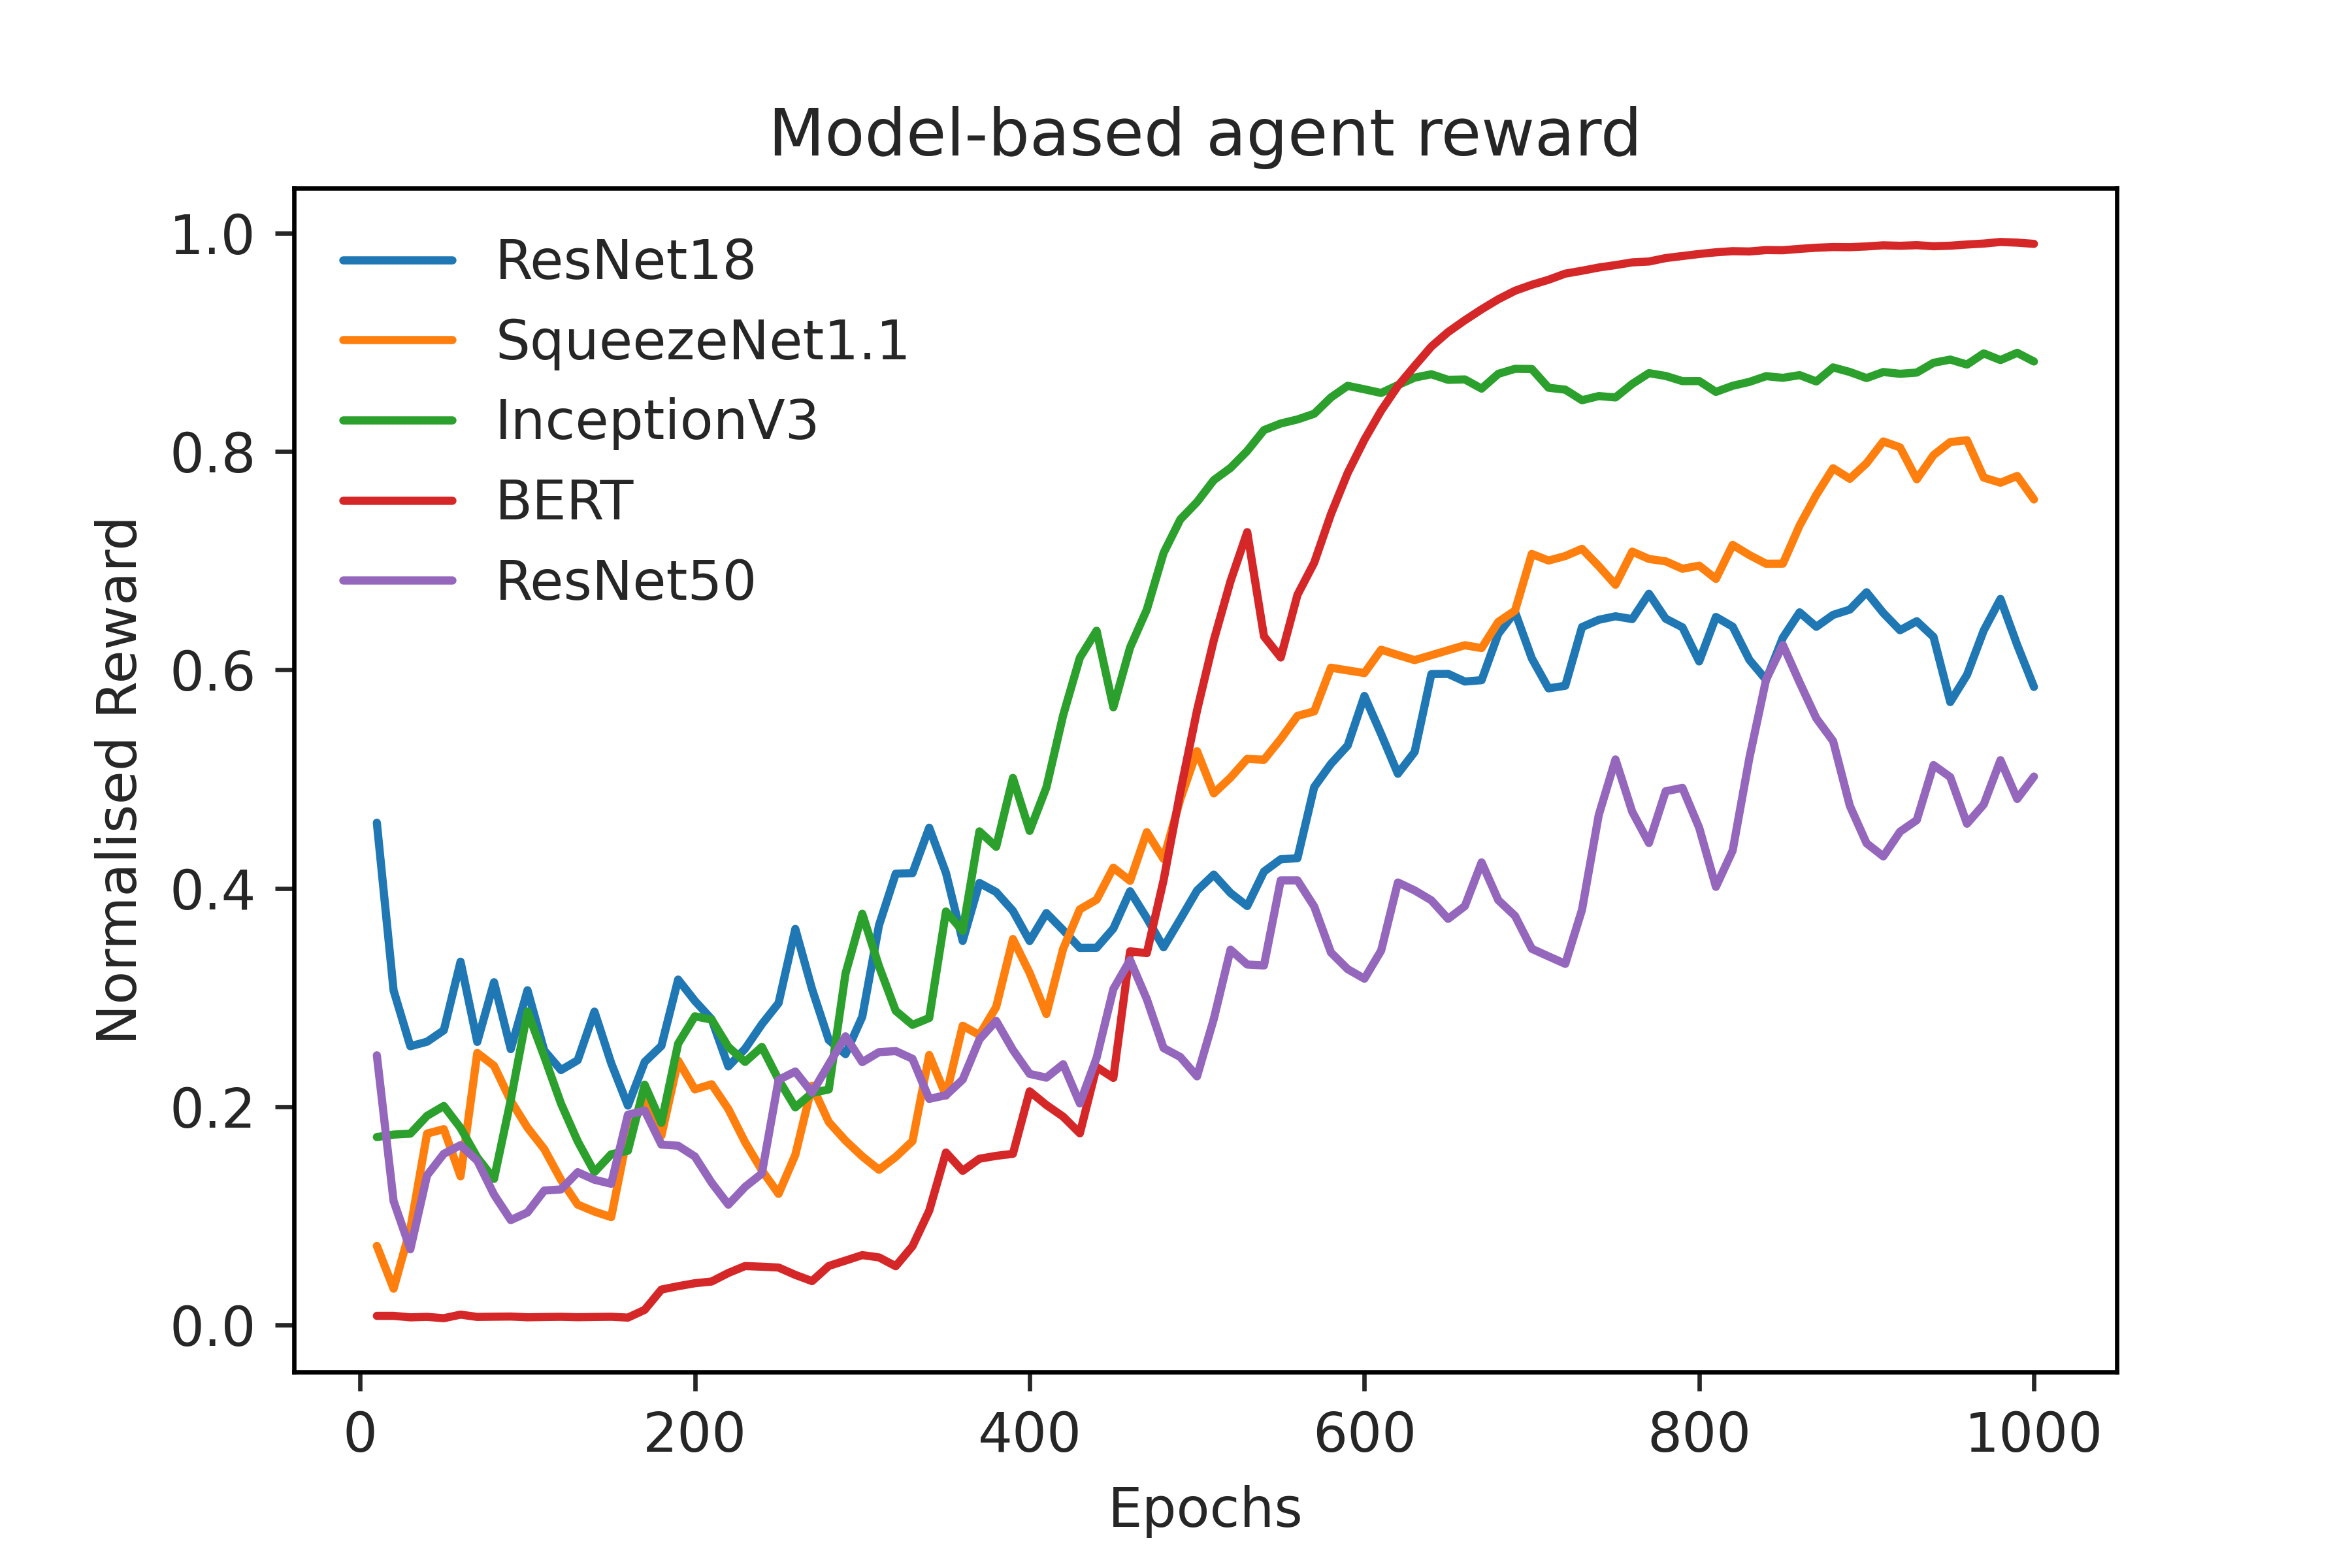
\includegraphics[width=1\columnwidth]{sections/5evaluation/images/mb_ctrl_training_reward}
  \caption[Predicted epoch reward during training of agent in world model]{Predicted reward produced by the world model while training the agent inside a the imagined environment. All rewards are normalised into the same range.}
  \label{fig:eval:world-model-pred-reward}
\end{figure}

Figure \ref{fig:eval:world-model-pred-reward} shows the reward (decrease in estimated runtime) for each graph as predicted by the world model during training. As the tested graphs have a wide range of epoch rewards, we perform min-max normalisation to scale the plots into the same range. We observe the same results as figure \ref{fig:eval:world-model-runtimes} in which the optimisations applied to BERT during training results in the optimal graph found after 700 epochs. On the other hand, graphs such as ResNet 18/50 are less stable during training with a high epoch to epoch variation in rewards. In comparison to the rewards received by the model-free agent during training, we note that the strictly model-free agent was more stable during training, and additionally, consistently found the optimised graph after approximately 1000 epochs.

\subsubsection{Discussion}

If we assume that both the model-free and model-based agents should achieve a similar level in performance once trained, the results in figure \ref{fig:eval:world-model-pred-reward} and \ref{fig:eval:mf-agent-reward} show that the agents trained in the world model are less stable with a higher reward variance. We hypothesise that there are three factors for such a discrepancy to occur:

\begin{itemize}
  \item Imperfect world-model reward predictions leading to incorrect (or invalid) actions being performed
  \item Next state prediction by the world-model generating states that are invalid due to poor generalisation of the model
  \item Incorrect action mask predictions that would lead to a divergence in between the world-model state and real environment state 
\end{itemize}

In an attempt to resolve the issues highlighted above, we performed further experiments which we believe would aid in both reducing the variance in reward prediction as well as stabilise the world-model during training to prevent state divergence over time. We performed a temperature sweep of the hyperparameter $\tau$ which is used in training agent inside the world model, shown in section \ref{sec:eval:subsec:temp-sweep}.

% Secondly, we also investigated splitting the prediction components of the world model such that we do not predict the next state, rewards, terminals and masks in a single model. Rather, we use a separate network to perform reward prediction using the hidden state, $h_t$ from the MDN-RNN as well as the latent graph state $s_t$.

% [TODO finish]


\subsubsection{Temperature Sweep}
\label{sec:eval:subsec:temp-sweep}

\begin{table}[htbp]
  \centering
  \begin{tabular}{@{}lll@{}}
  \toprule
  Temperature  & World-model Score        & Real Score                \\ \midrule
  0.1          & -6.67\% $\pm$ 0.6\%          & -43.92\% $\pm$ 5.1\%         \\
  0.5          & -7.75\% $\pm$ 0.3\%          & -55.33\% $\pm$ 6.7\%         \\
  0.75         & -9.10\% $\pm$ 0.4\%          & -55.80\% $\pm$ 5.2\%         \\
  1.0          & -8.85\% $\pm$ 1.2\%          & -55.78 $\pm$ 4.0\%           \\
  1.2          & -9.91\% $\pm$ 0.8\%          & -57.01\% $\pm$ 3.9\%         \\
  \textbf{1.5} & \textbf{-8.37\% $\mathbf{\pm}$ 0.6\%} & \textbf{-58.23\% $\mathbf{\pm}$ 3.6\%} \\
  1.75         & -9.92\% $\pm$ 1.0\%          & -52.07\% $\pm$ 5.8\%         \\
  2.0          & -9.65\% $\pm$ 0.8\%          & -46.12\% $\pm$ 5.4\%         \\
  2.5          & -10.04\% $\pm$ 2.0\%         & -41.14\% $\pm$ 10.2\%         \\
  3.0          & -10.38\% $\pm$ 1.9\%         & -51.32\% $\pm$ 7.2\%         \\ \bottomrule
  \end{tabular}
  \caption[Rewards using range of temperatures]{Temperature sweep of trained model-based agent optimising the BERT network. We ran each experiment five times and show both the average performance improvement as well as the variance between runs.}
  \label{table:eval:agent-temperatures}
\end{table}

Table \ref{table:eval:agent-temperatures} shows the results from performing a temperature sweep in which we used different values of $\tau$ while training the agent in a world model. After training, we evaluated the agent which produced an optimised graph that we evaluated to determine average runtime. The table shows the average reduction in runtime and standard deviation, averaged over five runs, compared to the unoptimised graph. The motivation for using a range of temperatures is that a higher value of $\tau$ leads to softer targets for the agent to predict, thereby improving generalisation. Conversely, a lower value of $\tau$ presents hard targets and thus when $\tau = 1.0$, it is equivalent to using the unmodified mixing weight, $\pi$, of the MDN.

Based upon the results in table \ref{table:eval:agent-temperatures} from the conducted experiments, we note that the world model agents are stable to temperatures within the range of $\tau = 0.5$ to $\tau = 1.75$. Although the runtime improvement world-model from the environment is consistently above 6\%, we observe a large difference between the predicted runtime improvement and the real environment reward.

% Despite the experiments performed in section [TODO] \ref{sec:eval:subsubsec:wm-acc} which shows a low MSE between the predicted and real scores, during evaluation we see a large divergence between the two scores. Therefore, we performed further experiments to evaluate the performance of the agents inside the world-model using a composite model in which the reward prediction is conducted in a separately trained network.

% [TODO include results from separate reward prediction network]

\subsubsection{Agent Convergence}
\label{sec:eval:subsec:agent-conv}

\begin{figure}[ht]
  \centering
  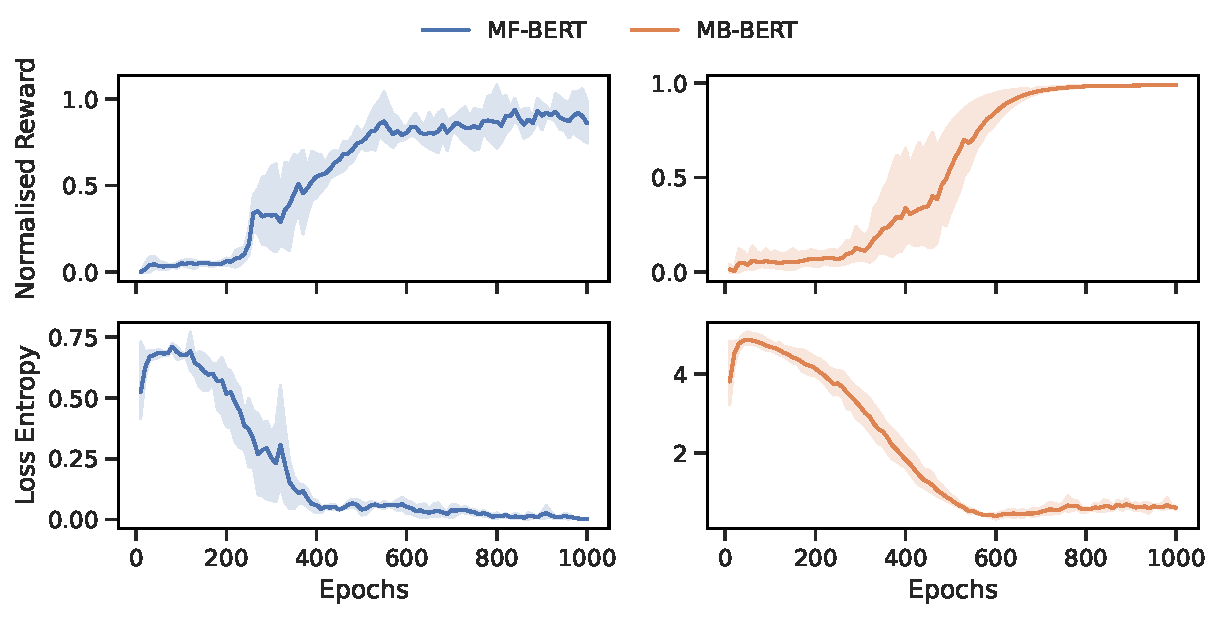
\includegraphics[width=1\columnwidth]{sections/5evaluation/images/agent_convergence.pdf}
  \caption[Convergence line plots of MF and MB approaches]{Agent reward and loss for model-free and model-based agents shown on the left (blue) and right (orange) respectively. We trained the agents on the BERT graph for 1000 epochs and repeated the experiments five times. We show the 95\% confidence interval in the shaded area of each plot.}
  \label{fig:eval:agent-mf-mb-convg}
\end{figure}

As we have previously claimed, there are many benefits to using a world model as the environment where we train the controller agent. In Figure \ref{fig:eval:agent-mf-mb-convg} we show the agent reward and loss during training for 1000 epochs on the BERT graph using model-free (MF) and model-based (MB) agents. Also, we used the results from our previous temperature sweep experiment by choosing the temperature $\tau = 1.5$ for use when training the controller. We found that the model-based agent, when trained using tuned hyperparameters, was more stable than the MF agent trained inside the real environment; the variance between runs was lower for the model-based agent compared to the MF agent. However, we found that the variance in the optimised runtime of the models produced by the MF agent was larger than the MB agent, with a variance of $6.1\%$ and $3.6\%$ respectively.


\subsubsection{Graph transformations}

\begin{figure}[ht]
  \centering
  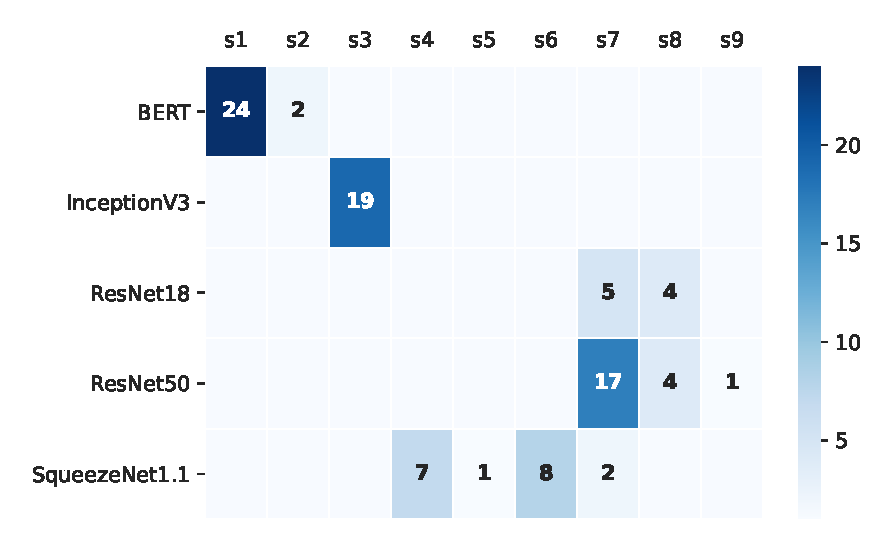
\includegraphics[width=1\columnwidth]{sections/5evaluation/images/xfer_heatmap}
  \caption[Heatmap of graph transformations applied by MB controller]{Heatmap showing the transformations applied by the trained controller acting inside the world model. Although there are over 100 possible transformations, we only show the transformations applied onto at least one graph. The counts for each transformation show the number of times it has been applied.}
  \label{fig:eval:xfer-heatmap}
\end{figure}

Figure \ref{fig:eval:xfer-heatmap} shows a heatmap of the various graph transformations which have been applied by a trained model-free agent during evaluation. Notably, the optimisations applied to the ResNet18/50 graphs apply similar transformations, those targeting the convolutions in the network; as the networks are composed of alike convolutional operators, with different depths, we apply analogous transformations. On the otherhand, for recurrent networks such as BERT, we only apply relatively few transformations. This is in stark contrast to the series of transformations found by TASO which applies four distinct substitutions in comparison to the two applied by our approach. Despite the large disparity in both the specific transformations as well as number of times we applied transformations, the performance difference between TASO and our proposed method is small.

\section{Discussion}
Throughout this chapter we have evaluated our claims which we formed in the introduction. We have provided the results to various experiments covering the reinforcement of our baseline measurements and those which show the performance of the proposed agents. Overall, we have found that our proposed approach outperforms the TensorFlow optimisation strategy on all graphs. However, in some cases, namely the deeper convolutional networks such as ResNet50 and InceptionV3, our agents failed to apply optimisations that outperform those performed by TensorRT and TASO.

In examining the model-based agent performance, we found that a world-model is able to accurately learn and simulate the transition dynamics of an environment, showing that despite the complex nature of the state-action transitions the world-model is flexible to learn its behaviour and adapt to previously unseen state-action pairs. 

Notably, although the state-action prediction and the terminal state prediction was accurate, we found the reward prediction had a large error when compared to the real reward produced by the environment. However, and surprisingly, this disparity between the two rewards did not have a significant impact on the agent performance as we showed in section \ref{sec:eval:subsec:temp-sweep}, the agent trained inside the world model is stable to a wide range of operating conditions.

Finally, the primary takeaway from these experiments is that reinforcement learning, especially model-based methods, are extremely powerful and can learn to model complex dynamic systems and provide important benefits. Nonetheless, we note that such methods still suffer instability during training, and imperfections in the world-model leads to agent exploitation of the faulty environment and therefore poor performance in the real environment---tuning of the world-model hyperparameters remains vital to producing a stable, performant agent. 
% TODO List:

% - Hyperparameter search

% - Reward prediction for model-based method (Separate reward pred network, compare MSE)

% - Show sample graph xfers graphically
